\begin{figure*}[t]
  \centering
  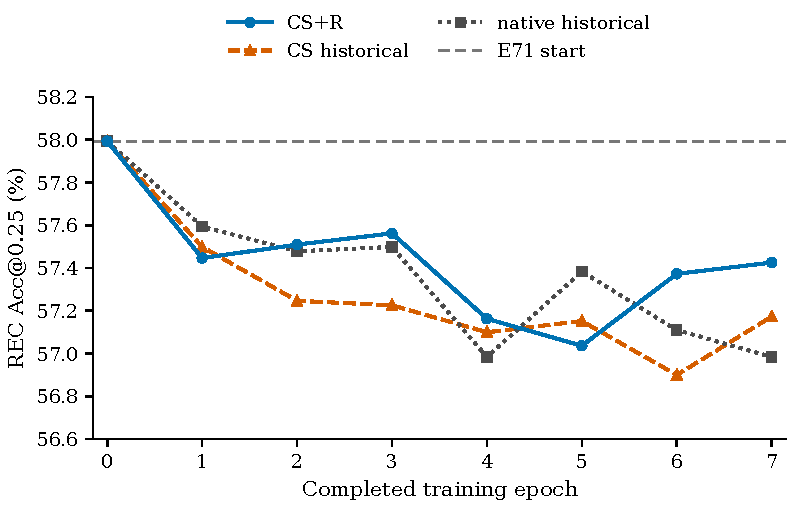
\includegraphics[width=0.8\textwidth]{r_epoch7_acc025.pdf}
  \caption{ScanRefer REC Acc@0.25 after zero through seven completed training epochs. Each point evaluates the same 9,508 expressions with the native last/bbs output, E71 initialization, seed 2027, and batch size 12. CS+R additionally uses deterministic M1 aggregation, so historical CS and native curves are descriptive references rather than an isolated R ablation. Epochs are correlated snapshots of one seed. The vertical axis is truncated; the E71 line is the zero-update result.}
  \label{fig:cs_readback_epoch7_acc025}
\end{figure*}

\begin{figure*}[t]
  \centering
  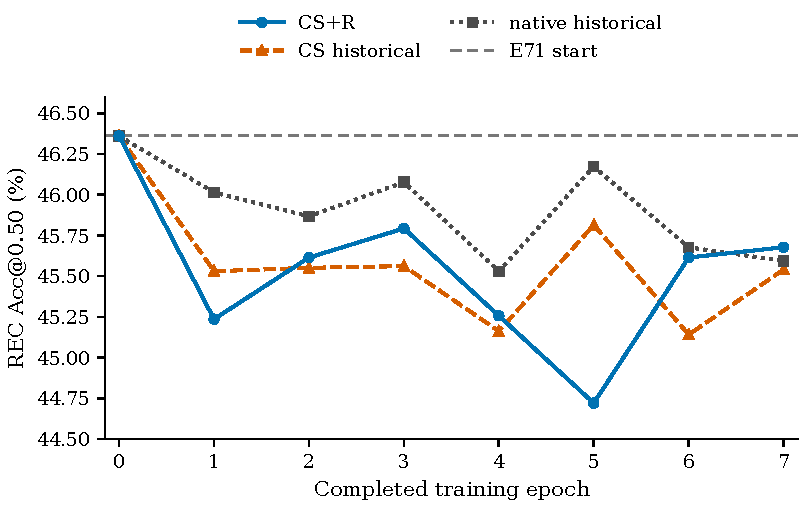
\includegraphics[width=0.8\textwidth]{r_epoch7_acc050.pdf}
  \caption{ScanRefer REC Acc@0.50 after zero through seven completed training epochs. Each point evaluates the same 9,508 expressions with the native last/bbs output, E71 initialization, seed 2027, and batch size 12. CS+R additionally uses deterministic M1 aggregation, so historical CS and native curves are descriptive references rather than an isolated R ablation. Epochs are correlated snapshots of one seed. The vertical axis is truncated; the E71 line is the zero-update result.}
  \label{fig:cs_readback_epoch7_acc050}
\end{figure*}
